\section{Methodology}
\label{sec:methods}

In this section, we detail our technical methodology for model evaluation, interpretability, and robustness assessment.

%-------------------------------------------------------------------------
\subsection{Comprehensive Method Development}
\label{sec:comp-method}

\subsubsection{Colour Histograms + HOG into Random Forest}
The first model we developed was a traditional Random Forest classifier with colour histograms and HOG features extracted to create unique feature vectors for each image. The random forest classifier is a standard baseline that has been used in previous papers to achieve accurate, generalisable results for image classification \cite{singh2018improved}. Therefore, it was chosen as one of the main traditional classifiers to compare our more advanced models against.

Colour histograms represent the global distribution of pixel colours in images, and provide a very intuitive way to understand the colour space of any image. For classifying fine-grained colourful visuals in mini-iNat2021, these colour histograms become vital providers of key discriminative information that allows the Random Forest classifier to differentiate different species classes via colour composition. For this task, HSV and L*a*b colour spaces were evaluated for the colour histograms as their channels are less
correlated than RGB. L*a*b was tested against HSV to determine whether a more perceptually uniform colour space would yield a more discriminative feature space for colour representation across species.

HOG features, in particular, capture shape and general appearance of the image through edge and contour information \cite{sen2026featureengineering}. Different species present different shapes and sizes, and so understanding these can help the classifier better distinguish between different species. Different cell pixel inputs were tested for the building of the HOGs primarily to examine whether smaller cells would yield finer-grained gradient information and therefore a more discriminative feature representation,
at the cost of a higher-dimensional feature vector.

Feeding both the colour histograms and the histograms of oriented gradients into the random forest classifier, therefore, creates an excellent, generalisable baseline with accurate colour discrimination and shape/appearance discrimination to compare against deep learning methods.

\subsubsection{BoVW--RootSIFT with Linear SVM}
\label{sec:method-svm}
Our second traditional approach represents each image with a Bag-of-Visual-Words (BoVW) histogram~\cite{csurka2004visual} built from RootSIFT descriptors and classifies it with a linear Support Vector Machine (SVM). Unlike the global colour and gradient statistics of the Random Forest, this is a second hand-crafted representation based on local structure, giving a further point of comparison against the learned deep features.
 
We use SIFT~\cite{lowe2004distinctive} because its local descriptors are robust to scale and orientation changes common in citizen-science photographs, and RootSIFT~\cite{arandjelovic2012three} as a near cost-free refinement whose normalisation makes Euclidean comparison approximate the Hellinger kernel. We pair the resulting histograms with a linear SVM~\cite{cortes1995support} because they are sparse and high-dimensional, a setting where linear classifiers perform well and scale to 40{,}000 training images across 1,000 classes. Keeping the classifier simple focuses the study on the quality of the representation.
 
Each ablation targets a known weakness of the plain histogram. Vocabulary size governs a granularity trade-off between merging distinct local structures and producing sparse, unstable histograms. Soft assignment addresses the quantisation error incurred by assigning each descriptor to a single word~\cite{vangemert2010visual}, a concern when species differ only in subtle detail. TF-IDF weighting tests whether words shared by most images are less discriminative here, and Spatial Pyramid Matching~\cite{lazebnik2006beyond} restores the spatial layout the plain histogram discards. We vary one choice at a time, combine the beneficial ones, and finally tune the SVM regularisation parameter $C$. All choices are made on validation macro-F1, which weights every species equally and exposes weak per-class behaviour that overall accuracy can hide. Implementation details appear in \cref{sec:trad-svm}.

\subsubsection{EfficientNet V2}
\label{sec:method-efficientnetv2}
Our first deep-learning model is \textbf{EfficientNetV2-S} \cite{tan2021efficientnetv2}. Following \cref{sec:litreview-efficientnetv2}, its Fused-MBConv and MBConv design provides an efficiency-oriented deep baseline with learned visual features beyond the hand-crafted representations used by the traditional pipelines. The S variant keeps multiple controlled experiments practical while retaining the capacity needed for fine-grained classification across 1,000 species.

The subset provides only 40 training images per species, motivating the transfer-learning comparison in \cref{sec:litreview-transfer}. We compare ImageNet-1K fine-tuning and training from scratch under matched no-augmentation and full-augmentation settings. Each regime uses the training schedule appropriate to fine-tuning or learning from random initialization, so the comparison evaluates the practical value of a generic visual prior when task-specific supervision is limited.

Following \cref{sec:litreview-training-strategies}, the cumulative augmentation ablation adds Crop, Flip, and Color Jitter one at a time to identify each component's contribution. Intermediate levels are evaluated in the pretrained regime, while the scratch regime uses the two endpoints to measure the full pipeline's effect within the available compute budget. Within each initialization regime, optimization and regularization are held fixed across augmentation levels, allowing performance changes to be associated with augmentation. The implementation details are reported in \cref{sec:dl-efficientnetv2}.

\subsubsection{ConvNeXt V2}
\label{sec:method-convnextv2}
We selected \textbf{ConvNeXt V2} \cite{woo2023convnextv2} over a Transformer backbone for this study specifically because: (i) its convolutional inductive bias is well-suited to our computational resource constraints and the relatively small size of our subsampled dataset (40,000 training images), and (ii) its compatibility with fully-convolutional, gradient-based interpretability methods such as Grad-CAM (\cref{sec:adv-method}).

Fine-tuning and from-scratch training utilize standard optimization strategies inspired by \cref{sec:litreview-training-strategies}; specific hyperparameter configurations and schedules are detailed in \cref{sec:suppl-convnextv2-hyperparams}.

Motivated by \cref{sec:litreview-training-strategies}, we ablate augmentation and regularization for ConvNeXt V2 in stages. Training begins from a shared Basic transform stack---random resized cropping, horizontal flipping, and colour jitter---after which the from-scratch runs successively enable DropPath, CoarseDropout, and CutMix/MixUp so that each addition can be assessed in isolation. The pretrained comparison is limited to the None and Basic endpoints, whereas the fuller ladder is reserved for training from scratch. Aside from the DropPath rate and warmup schedule, which are themselves ablated, other optimization choices remain unchanged within each initialization setting. Details of the experimental setup appear in \cref{sec:dl-convnextv2}.

%-------------------------------------------------------------------------
\subsection{Advanced Method Development}
\label{sec:adv-method}
We conduct two advanced studies on our best-performing ConvNeXt V2 model to evaluate visual interpretability and environmental robustness.

\subsubsection{Grad-CAM Interpretability}
To analyze spatial feature importance, we implement Grad-CAM \cite{selvaraju2017grad} targeted at stage 4's final depthwise conv layer (\texttt{dwconv}). For feature activation tensor $\mathbf{A} \in \mathbb{R}^{C \times H \times W}$ ($C=768, H=7, W=7$) captured via PyTorch hooks, channel importance weights $\alpha_k^c$ and coarse heatmap $L_{\text{Grad-CAM}}^c$ are computed as:
\begin{equation}
  \alpha_k^c = \frac{1}{H \times W} \sum_{i=1}^{H} \sum_{j=1}^{W} \frac{\partial Y^c}{\partial A_{i,j}^k}
\end{equation}
\begin{equation}
  L_{\text{Grad-CAM}}^c = \text{ReLU}\left( \sum_{k=1}^{C} \alpha_k^c \mathbf{A}^k \right)
\end{equation}
The single-channel heatmap is normalized to $[0, 1]$, bilinearly interpolated to input resolution, and blended with a \texttt{jet} colormap ($\alpha = 0.4$).

\subsubsection{Robustness to Image Degradation}
\label{sec:robustness-method}
Following ImageNet-C principles \cite{hendrycks2019robustness}, we evaluate test-set performance under 4 corruption types across 5 severity levels ($s \in \{0, 1, 2, 3, 4\}$, with $s=0$ as baseline):
\begin{itemize}[noitemsep,topsep=0pt]
  \item \textbf{Additive Gaussian Noise}: $\mathbf{I}_{\text{noisy}} = \text{clip}(\mathbf{I} + \mathbf{N}, 0, 1)$ where $\mathbf{N} \sim \mathcal{N}(0, \sigma^2)$ with $\sigma = 0.05 s$.
  \item \textbf{Gaussian Blur}: 2D isotropic Gaussian filter with blur radius $r = 1.0 s$ pixels.
  \item \textbf{Motion Blur}: Diagonal motion kernel $\mathbf{K} \in \mathbb{R}^{L \times L}$ ($L = 4s + 1$, $K_{i,j} = \frac{1}{L}\delta_{i,j}$) applied via depthwise conv2d.
  \item \textbf{JPEG Compression}: Encoded via PIL with quality $q(s) \in \{100, 50, 25, 10, 5\}$ for severity levels $s \in \{0, 1, 2, 3, 4\}$.
\end{itemize}

\begin{figure*}[t]
  \centering
  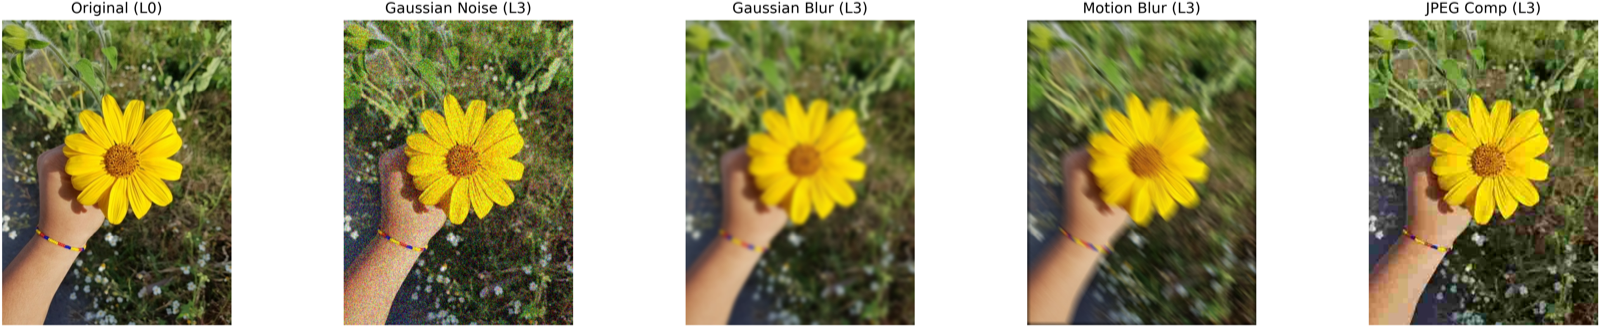
\includegraphics[width=0.7\linewidth]{image/robustness_analysis/degradation_examples.png}
  \caption{\textbf{Visual demonstration of the 4 image degradation types at Severity Level 3.} From left to right: \textit{Original Image} ($s=0$), \textit{Additive Gaussian Noise} ($\sigma=0.15$), \textit{Gaussian Blur} ($r=3.0$), \textit{Motion Blur} ($L=13$), and \textit{JPEG Compression} ($q=10$).}
  \label{fig:degradation_examples}
\end{figure*}
